\documentclass[a4paper,12pt]{article}
\usepackage[utf8]{inputenc}
\usepackage[T1]{fontenc}
\usepackage[margin=1in]{geometry}
\usepackage{setspace}
\usepackage{titlesec}
\usepackage{inconsolata}
\usepackage{graphicx}

\usepackage{color}

\definecolor{pblue}{rgb}{0.13,0.13,1}
\definecolor{pgreen}{rgb}{0,0.5,0}
\definecolor{pred}{rgb}{0.9,0,0}
\definecolor{pgrey}{rgb}{0.46,0.45,0.48}

\usepackage{listings}
\lstset{language=Java,
  showspaces=false,
  showtabs=false,
  breaklines=true,
  showstringspaces=false,
  breakatwhitespace=true,
  commentstyle=\color{pgreen},
  keywordstyle=\color{pblue},
  stringstyle=\color{pred},
  basicstyle=\ttfamily,
  moredelim=[il][\textcolor{pgrey}]{$$},
  moredelim=[is][\textcolor{pgrey}]{\%\%}{\%\%}
}
% Title and author
\title{TP5 - Etude et amélioration d’une application}
\author{Jesimiel Manza}
\date{\today}

\begin{document}

\maketitle

\section*{Abstract}
% Your abstract goes here.

\section{Introduction}
Dans ce TP, nous allons nous interesser sur une application permettant de simuler la vie d'une colonie de fourmis peintres. Les fourmis se déplacent sur un surface sans bord.Le déplacement d’une fourmi obéit à des règles simples : soit elle détecte à proximité une couleur qui l’intéresse et décide de la suivre ou pas, soit elle se déplace aléatoirement. A chaque déplacement, la fourmi dépose sa couleur sur la surface. Sur une exécution longue, une auto-organisation apparaît. 
L'objectif de ce TP est d'analyser les performances de l'application existante et les faiblesse du code. Lorsque cette permière partie de vérification 

\section{Présentation de l'application}
% Your literature review goes here.

\section{Amélioration}

\subsection{CPainting}
\subsubsection{init}
\begin{lstlisting}
    public void init() {
        int i, j;
        mGraphics = getGraphics();
        synchronized (mMutexCouleurs) {
          mGraphics.clearRect(0, 0, mDimension.width, mDimension.height);
    
          // initialisation de la matrice des couleurs
    
          for (i = 0; i != mDimension.width; i++) {
            for (j = 0; j != mDimension.height; j++) {
              mCouleurs[i][j] = new Color(mCouleurFond.getRed(), mCouleurFond.getGreen(), mCouleurFond.getBlue());
            }
          }
        }
    
        // initialisation de la matrice de convolution : lissage moyen sur 9
        // cases
        
        /*
         * 1 2 1 2 4 2 1 2 1
         */
        CPainting.mMatriceConv9[0][0] = 1 / 16f;
        CPainting.mMatriceConv9[0][1] = 2 / 16f;
        CPainting.mMatriceConv9[0][2] = 1 / 16f;
        CPainting.mMatriceConv9[1][0] = 2 / 16f;
        CPainting.mMatriceConv9[1][1] = 4 / 16f;
        CPainting.mMatriceConv9[1][2] = 2 / 16f;
        CPainting.mMatriceConv9[2][0] = 1 / 16f;
        CPainting.mMatriceConv9[2][1] = 2 / 16f;
        CPainting.mMatriceConv9[2][2] = 1 / 16f;
    
        // initialisation de la matrice de convolution : lissage moyen sur 25
        // cases
        /*
         * 1 1 2 1 1 1 2 3 2 1 2 3 4 3 2 1 2 3 2 1 1 1 2 1 1
         */
        CPainting.mMatriceConv25[0][0] = 1 / 44f;
        CPainting.mMatriceConv25[0][1] = 1 / 44f;
        CPainting.mMatriceConv25[0][2] = 2 / 44f;
        CPainting.mMatriceConv25[0][3] = 1 / 44f;
        CPainting.mMatriceConv25[0][4] = 1 / 44f;
        CPainting.mMatriceConv25[1][0] = 1 / 44f;
        CPainting.mMatriceConv25[1][1] = 2 / 44f;
        CPainting.mMatriceConv25[1][2] = 3 / 44f;
        CPainting.mMatriceConv25[1][3] = 2 / 44f;
        CPainting.mMatriceConv25[1][4] = 1 / 44f;
        CPainting.mMatriceConv25[2][0] = 2 / 44f;
        CPainting.mMatriceConv25[2][1] = 3 / 44f;
        CPainting.mMatriceConv25[2][2] = 4 / 44f;
        CPainting.mMatriceConv25[2][3] = 3 / 44f;
        CPainting.mMatriceConv25[2][4] = 2 / 44f;
        CPainting.mMatriceConv25[3][0] = 1 / 44f;
        CPainting.mMatriceConv25[3][1] = 2 / 44f;
        CPainting.mMatriceConv25[3][2] = 3 / 44f;
        CPainting.mMatriceConv25[3][3] = 2 / 44f;
        CPainting.mMatriceConv25[3][4] = 1 / 44f;
        CPainting.mMatriceConv25[4][0] = 1 / 44f;
        CPainting.mMatriceConv25[4][1] = 1 / 44f;
        CPainting.mMatriceConv25[4][2] = 2 / 44f;
        CPainting.mMatriceConv25[4][3] = 1 / 44f;
        CPainting.mMatriceConv25[4][4] = 1 / 44f;
    
        // initialisation de la matrice de convolution : lissage moyen sur 49
        // cases
        /*
         * 1 1 2 2 2 1 1 1 2 3 4 3 2 1 2 3 4 5 4 3 2 2 4 5 8 5 4 2 2 3 4 5 4 3 2 1 2
         * 3 4 3 2 1 1 1 2 2 2 1 1
         */
        CPainting.mMatriceConv49[0][0] = 1 / 128f;
        CPainting.mMatriceConv49[0][1] = 1 / 128f;
        CPainting.mMatriceConv49[0][2] = 2 / 128f;
        CPainting.mMatriceConv49[0][3] = 2 / 128f;
        CPainting.mMatriceConv49[0][4] = 2 / 128f;
        CPainting.mMatriceConv49[0][5] = 1 / 128f;
        CPainting.mMatriceConv49[0][6] = 1 / 128f;
    
        CPainting.mMatriceConv49[1][0] = 1 / 128f;
        CPainting.mMatriceConv49[1][1] = 2 / 128f;
        CPainting.mMatriceConv49[1][2] = 3 / 128f;
        CPainting.mMatriceConv49[1][3] = 4 / 128f;
        CPainting.mMatriceConv49[1][4] = 3 / 128f;
        CPainting.mMatriceConv49[1][5] = 2 / 128f;
        CPainting.mMatriceConv49[1][6] = 1 / 128f;
    
        CPainting.mMatriceConv49[2][0] = 2 / 128f;
        CPainting.mMatriceConv49[2][1] = 3 / 128f;
        CPainting.mMatriceConv49[2][2] = 4 / 128f;
        CPainting.mMatriceConv49[2][3] = 5 / 128f;
        CPainting.mMatriceConv49[2][4] = 4 / 128f;
        CPainting.mMatriceConv49[2][5] = 3 / 128f;
        CPainting.mMatriceConv49[2][6] = 2 / 128f;
    
        CPainting.mMatriceConv49[3][0] = 2 / 128f;
        CPainting.mMatriceConv49[3][1] = 4 / 128f;
        CPainting.mMatriceConv49[3][2] = 5 / 128f;
        CPainting.mMatriceConv49[3][3] = 8 / 128f;
        CPainting.mMatriceConv49[3][4] = 5 / 128f;
        CPainting.mMatriceConv49[3][5] = 4 / 128f;
        CPainting.mMatriceConv49[3][6] = 2 / 128f;
    
        CPainting.mMatriceConv49[4][0] = 2 / 128f;
        CPainting.mMatriceConv49[4][1] = 3 / 128f;
        CPainting.mMatriceConv49[4][2] = 4 / 128f;
        CPainting.mMatriceConv49[4][3] = 5 / 128f;
        CPainting.mMatriceConv49[4][4] = 4 / 128f;
        CPainting.mMatriceConv49[4][5] = 3 / 128f;
        CPainting.mMatriceConv49[4][6] = 2 / 128f;
    
        CPainting.mMatriceConv49[5][0] = 1 / 128f;
        CPainting.mMatriceConv49[5][1] = 2 / 128f;
        CPainting.mMatriceConv49[5][2] = 3 / 128f;
        CPainting.mMatriceConv49[5][3] = 4 / 128f;
        CPainting.mMatriceConv49[5][4] = 3 / 128f;
        CPainting.mMatriceConv49[5][5] = 2 / 128f;
        CPainting.mMatriceConv49[5][6] = 1 / 128f;
    
        CPainting.mMatriceConv49[6][0] = 1 / 128f;
        CPainting.mMatriceConv49[6][1] = 1 / 128f;
        CPainting.mMatriceConv49[6][2] = 2 / 128f;
        CPainting.mMatriceConv49[6][3] = 2 / 128f;
        CPainting.mMatriceConv49[6][4] = 2 / 128f;
        CPainting.mMatriceConv49[6][5] = 1 / 128f;
        CPainting.mMatriceConv49[6][6] = 1 / 128f;
    
        mSuspendu = false;
      }
\end{lstlisting}
La création de matrice n'est vraiment pas optimale. En moyenne, en utilisant le fichier html de base, il y a 430676 fourmis qui circulent. 

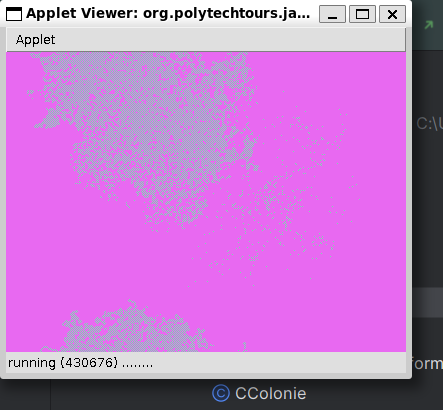
\includegraphics[scale=0.75]{images/appletSansModification.png}

\section{Analyse finale}
% Your results go here.

\section{Discussion}
% Your discussion goes here.

\section{Conclusion}
% Your conclusion goes here.

\section*{Acknowledgments}
% Your acknowledgments (if any) go here.

\begin{thebibliography}{9}
    % Your bibliography goes here.
\end{thebibliography}

\end{document}
